\chapter{Derivadas en física}

\begin{tikzpicture}
	\fill [left color=red!50, right color=teal!50] (0,0) rectangle (6.5,.2);
	\fill [left color=teal!50, right color=blue!50] (6.5,0) rectangle (11.5,.2);
	\end{tikzpicture}


\begin{comment}
\vspace{1cm}
\section{Uno.Uno}

\begin{tikzpicture}
	\fill [left color=red!50, right color=teal!50] (0,0) rectangle (3.5,.1);
	\fill [left color=teal!50, right color=blue!50] (3.5,0) rectangle (7.5,.1);
	\end{tikzpicture}
\vspace{0.5cm}

\vspace{1cm}
\subsection{Uno.Uno.Uno}
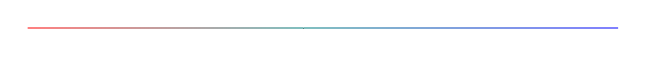
\begin{tikzpicture}
	\fill [left color=red!50, right color=teal!50] (0,0) rectangle (3.5,.01);
	\fill [left color=teal!50, right color=blue!50] (3.5,0) rectangle (7.5,.01);
	\end{tikzpicture}
\vspace{0.5cm}

\end{comment}


\vspace{1cm}
\section{La diferencial en física}

\begin{tikzpicture}
	\fill [left color=red!50, right color=teal!50] (0,0) rectangle (3.5,.1);
	\fill [left color=teal!50, right color=blue!50] (3.5,0) rectangle (7.5,.1);
	\end{tikzpicture}
\vspace{0.5cm}

\setlength{\parindent}{0cm}

\begin{destacado}
\emph{``Un \textbf{diferencial} de una magnitud es una cantidad muy pequeña (infinitesimal) de dicha magnitud.''} 
\end{destacado}

Pero, ?`cómo de pequeña ha de ser la cantidad para considerarla un \emph{diferencial}?\footnote{Diferencial, infinitesimal o infinitésimo, frente a infinito, son números (hiperreales) que, sin ser cero, son menores  en valor absoluto que cualquier número real positivo. $\quad$ Matemáticamente, $\ \ A \text { infinitesimal si }\displaystyle \lim_{t\to 0}{A(t)}=0$ } Pues depende, el concepto diferencial ha de ser siempre en relación a los valores típicos que presente la variable en el campo de estudio. Por ejemplo, la cantidad de $1$ metro, en el sistema de estudio del movimiento de la tierra alrededor del sol sí puede ser considerada una cantidad diferencial pero no si el sistema en estudio son los sucesivos rebotes de una pelota dejada caer desde una mesa.

Si tenemos una magnitud que es función de varias variables, $f(x,y,\cdots)$, y estas sufren pequeños cambios diferenciales $x\to x+\dd x,\ y\to y+\dd y,\cdots $ entones, el cambio de nuestra magnitud será:
$\dd f=f(x+\dd x ,y+\dd y, \cdots) - f(x,y,\cdots)$


$\centerdot\ \ $ Si nuestra función es suma (resta) de otras dos,

$\qquad f=u+v  \ \to \ \left\{ 
\begin{matrix}  \ u\to u+\dd u \\ \ v\to v+\dd v  \end{matrix} 
\right. \quad \Rightarrow \ \boldsymbol{\dd f} = (u+\dd u)+(v+\dd v)- (u+ v)= \boldsymbol{ \dd u + \dd v }$	

$\centerdot \ \ $ Si nuestra función es producto de otras dos,

$\qquad f=u\, v  \ \to \ \left\{ 
\begin{matrix}  \ u\to u+\dd u \\ \ v\to v+\dd v  \end{matrix} 
\right. \quad \Rightarrow \ \boldsymbol{\dd f} = (u+\dd u)\ (v+\dd v)- (u\,v)= $

$\qquad =\cancel{u\, v} + u\dd v +v\dd u +\cancelto{0\ (*)}{ \dd u\, \dd v } - \cancel{u\, v}= \boldsymbol{ u\dd v +v\dd u}$	

\textcolor{gris}{
$(*) \qquad $ Si, por ejemplo, $\dd u \sim 10^{-3}$ y $\dd v \sim 10^{-3} \ \to \ \dd u\, \dd v  \sim 10^{-6}$, despreciable frente a los anteriores, se le llama diferencial de orden dos.}

Cuando el resultado de una operación sea suma de varios diferenciales, en primera aproximación, los diferenciales de orden superior al primero son despreciables frente a estos (producto de dos diferenciales es un diferencial de orden dos, el producto de tres de ellos es un diferencial de orden tres, etc.)

\emph{Dimensionalmente}, un diferencial tiene las mismas unidades de la magnitud de la que proviene.



\vspace{1cm}
\section{La derivada en física}

\begin{tikzpicture}
	\fill [left color=red!50, right color=teal!50] (0,0) rectangle (3.5,.1);
	\fill [left color=teal!50, right color=blue!50] (3.5,0) rectangle (7.5,.1);
	\end{tikzpicture}
\vspace{0.5cm}

\subrayado{\emph{``Una \textbf{derivada} en física es un cociente entre dos diferenciales (cantidades muy pequeñas'')}.}

\begin{figure}[H]
	\centering
	\includegraphics[width=.6\textwidth]{imagenes/T02IM01.png}
\end{figure}


Muchas leyes de la Física, la Química, la Biología o la Economía, son funciones que relacionan una variable `dependiente' y con otra variable `independiente' $x$, lo que suele escribirse en la forma $y = f(x)$. Si la variable independiente cambia de un valor inicial $x_0$ a otro $x$, la variable y lo hace de $f(x_0)$ a $f(x)$. La razón de cambio promedio o `tasa de variación media' de $y = f(x)$ con respecto a $x$ en el intervalo $[x_0,x]$ es: $\dfrac{\Delta f}{\Delta x}=\dfrac{f(x)-f(x_0)}{x-x_0}$

Con frecuencia interesa considerar la razón de cambio en intervalos cada vez más pequeños. Esto lleva a definir lo que podemos llamar `razón de cambio instantáneo' o `tasa de variación instantánea' de $y = f(x)$ con respecto a $x$ en el punto $x_0$ como: 
$\displaystyle \lim_{x\to x_0} \dfrac{f(x)-f(x_0)}{x-x_0} =\dfrac {\dd f}{\dd x}=f'(x)$

Un ejemplo clásico es la velocidad instantánea $v(t)$ en contraposición a la velocidad media $\bar v = \dfrac{\Delta x}{\Delta t}$, definida como:
$\quad  \displaystyle \boldsymbol{ v(t)= \dv{x}{t} } \ =\lim_{\Delta t\to 0} \dfrac{\Delta x}{\Delta t}$

En matemáticas, $\quad f(u)\ \to \ \displaystyle \dv{f}{u}=\dfrac{f(u+\dd u)-f(u)}{\dd u}= \ \mqty [ \dd u = h \\ h \to 0] \ = \lim_{h\to 0} \dfrac {f(u+h)-f(u)}{h}=f'(u)\ . \  \ $ Geométricamente coincide con la pendiente de la recta tangente a la función en el punto en que se calcule.

En física se suele usar la notación de Leibniz, $\displaystyle \dv{f}{u}$ preferiblemente a la de Lagrange $f'(u)$. \textcolor{gris}{Aún se usa otra notación en física, cuando la variable sobre la que se deriva es el tiempo $t$ es frecuente usar la notación de Newton $\dot f(t)=\displaystyle \dv{f}{t}=f'(t)$}

En la notación de Leibniz, tan importante es la magnitud a derivar como aquella respecto de la cual se deriva. $\displaystyle \ \dv{f}{u}\ $ se lee como \emph{derivada de $f$ respecto de $u$}.

\vspace{3mm} Puesto que $\qquad \qquad \displaystyle \subrayado{\ \boxed{\ \boldsymbol{ \dv{f}{u}=f'(u)} \ } \ } \qquad \to \qquad \subrayado{\  \boxed{ \ \boldsymbol{ \dd f \ = \ f'(u)\, \dd u } \ } \ }\ ,$

que pone de manifiesto la \emph{\textbf{relación entre derivada y diferencial.}}

\vspace{3mm} \textcolor{gris}{Al igual que un diferencial no siempre es la variación de una variable, p.e. $\dd V=\dd x\, \dd y\, \dd z$ es el producto de tres diferenciales de variables distintas, del mismo modo  no siempre un cociente de diferenciales será una derivada, $\rho=\dd m/\dd V$, la densidad no es la derivada de la masa respecto del volumen. Si la densidad no es constante, un pequeño elemento de volumen $\dd V$ tendrá una pequeña masa $\dd m$ que determinarán su densidad  $\rho=\dd m/\dd v$.}

\vspace{3mm} Dimensionalmente, al ser la derivada un cociente entre diferenciales, las unidades de la derivada son el cociente entre las unidades del \emph{numerador} y las del \emph{denominador}: 

$\quad \displaystyle \left[ \dv{f}{u} \right]=\dfrac{[f]}{[u]};
 \qquad [v]=\dfrac{[\dd x]}{[\dd t]}=\dfrac {\mathrm{m}}{\mathrm{s}}=\mathrm{m\, s}^{-1}$ 


\vspace{1cm}
\subsection{Álgebra de derivadas}
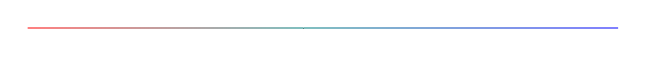
\begin{tikzpicture}
	\fill [left color=red!50, right color=teal!50] (0,0) rectangle (3.5,.01);
	\fill [left color=teal!50, right color=blue!50] (3.5,0) rectangle (7.5,.01);
	\end{tikzpicture}
\vspace{0.5cm}


\ul{Suma y producto}: 

$\quad \displaystyle \dv{(u+v)}{t}=\dfrac{\dd u + \dd v}{\dd t}=\dv{u}{t}+\dv{v}{t}$
$\qquad \qquad $
$\displaystyle \dv{(u\, v)}{t}=\dfrac{\dd u \, v+ u\, \dd v}{\dd t}=\dv{u}{t}\, v+ u\, \dv{v}{t}$

\vspace{5mm} Para \ul{magnitudes vectoriales}: 

$\quad	\overrightarrow A=A_x\vec i+A_y\vec j+A_z\vec k \quad \to \quad \displaystyle \dv{\overrightarrow A}{t}=\dv{A_x}{t}\vec i+\dv{A_y}{t}\vec j+\dv{A_z}{t}\vec k $


$\quad \displaystyle \dv{(\lambda \overrightarrow A)}{t}=\dv{\lambda}{t}\overrightarrow A+\lambda \dv{\overrightarrow A}{t};$

$\quad  \displaystyle  \dv{t} (\overrightarrow A \cdot \overrightarrow B)= \dv{\overrightarrow A}{t} \cdot \overrightarrow B + \overrightarrow A \cdot \dv{\overrightarrow B}{t}; \qquad \dv{t} (\overrightarrow A \times \overrightarrow B)= \dv{\overrightarrow A}{t} \times \overrightarrow B + \overrightarrow A \times \dv{\overrightarrow B}{t}$

\vspace{2mm} \textcolor{gris}{$\quad \overrightarrow A \cdot \overrightarrow  B \text{ producto escalar,} \quad \overrightarrow A \times \overrightarrow  B \text{ producto vectorial}$}

\vspace{5mm} Función compuesta, \ul{regla de la cadena}:

$A(x),\ x(t) \quad \to \qquad \displaystyle \dv{A}{t}=\dv{A}{x}\, \dv{x}{t}$
$\qquad \qquad \qquad $
$A(u),\, u(x),\,  x(t) \quad \to \qquad \displaystyle \dv{A}{t}=\dv{A}{u}\,  \dv{u}{x}\, \dv{x}{t}$

\vspace{5mm} Derivada de la \underline{función inversa}:

En notación de Lagrange: $\ 	\displaystyle \left( f^{-1} \right)\, ' \ = \ \dfrac 1{f'(f^{-1}(x))}\, ; \ \ $ en notación de Leibniz: $\ \ \displaystyle \dv{y}{x} \ = \ \dfrac{1}{\displaystyle \dv{x}{y}}$

\vspace{5mm} \ul{Derivadas de orden superior}:
$\quad \displaystyle \dv{t}\, \dv{A}{t}= \dv[2]{A}{t}=A''(t)=\ddot A(t) \ ; \qquad \  \dv{t}\, \dv[2]{A}{t}=\dv[3]{A}{t}\, ; \qquad \dv[n]{A}{t} $

Se leen, respectivamente, `derivada segunda de $A$ respecto de $t$ dos veces, derivada tercera de $A$ respecto de $t$ tres veces, derivada enésima de $A$ respecto de $t$ $n$ veces'.

No confundir $\quad \displaystyle \dv[2]{A}{t} \neq \left( \dv{A}{t} \right)^2\, , \ $ son incluso dimensionalmente cosas distintas: 

\textcolor{gris}{$\displaystyle \left[ \dv[2]{A}{t}  \right]=\dfrac{[A]}{[t^2]} \ \neq \ \dfrac{[A^2]}{[t^2]} = \left[ \left( \dv{A}{t} \right)^2 \right]\quad $ Por ejemplo, $\ \displaystyle a=\dv{v}{t}=\dv{t} \left( \dv{x}{t} \right) = \dv[2]{x}{t} \ \to \ \dfrac {\mathrm{m}}{\mathrm{s}^2} \ \ \bcancel{\cancel{ \dfrac {\mathrm{m}^2}{\mathrm{s}^2} }}$}

\vspace{1cm}
\color{ForestGreen!80}
\rule{250pt}{0.2pt}


\textsf{Leibniz fue quién mejor comprendió la importancia de una buena elección de los símbolos a usar en matemáticas, una vez introducida una notación la experimentaba durante mucho tiempo e incluso mantenía discusiones al respecto con sus colegas.}

\textsf{Leibniz, al límite del cociente incremental de una función en un punto (derivada), $\displaystyle \lim_{\Delta x \to 0} {\Delta f}/{\Delta x}$ le llamaba cociente de de diferenciales $\displaystyle \dd f  / \dd x$.}

\textsf{No solo era distinta la notación sino la forma de pensar. Leibniz pensaba, en lugar de límite de cantidades incrementales, que la derivada se obtenía cuando se pasaba de estas a cantidades incrementales a las cantidades \emph{diferenciales} siendo la \emph{derivada un cociente diferencial}, los incrementos $\Delta x,\, \Delta y$, al calcular la derivada se transformaban en \emph{infinitesinales} $\dd x,\, \dd y$, un \emph{nuevo tipo de números reales, que sin ser cero, son más pequeños en valor absoluto que cualquier número real positivo}.}

\textsf{Cauchy (s.XIX) abandonó el concepto de infinitesimales aunque se siguen usando en matemáticas aplicadas. La notación de Leibniz tiene la ventaja  de simplificar las operaciones y sus fórmulas se recuerdan sin dificultad.}

\vspace{-8mm}
\begin{flushright}
\rule{250pt}{0.2pt}		
\end{flushright}

	
\color{black}





\vspace{1cm}
\section{Derivadas parciales}

\begin{tikzpicture}
	\fill [left color=red!50, right color=teal!50] (0,0) rectangle (3.5,.1);
	\fill [left color=teal!50, right color=blue!50] (3.5,0) rectangle (7.5,.1);
	\end{tikzpicture}
\vspace{0.5cm}

Es muy frecuente que al estudiar determinadas magnitudes éstas dependan de varias variables: \emph{funciones de varias variables}.
\emph{ {La \textbf{derivada parcial} de una función $f(x,y,\cdots)$ respecto de una de ellas, p.e. la $x$, se obtiene derivando la expresión de $f$ respecto de  $x$ de modo usual solo que considerando que el resto de las variables son constantes}.} 
Se denota por $\displaystyle \pdv{f}{x}$ y se lee \emph{derivada parcial de $f$ respecto de $x$}.


Así, se habla de $\quad f(x,y,z,\cdots )\quad \to \quad\displaystyle \pdv{f}{x},\ \pdv{f}{y},\ \pdv[2]{f}{x}{y},\ \pdv[2]{f}{x},\ $ etc.

\vspace{5mm}\textcolor{gris}{$\triangleright \quad \ \text{ si } \ f(x,y)=x^2+3xy^2+2y^3 \ \quad \to \ \quad 
\displaystyle \pdv{f}{x}=2x+3y^2,\qquad \pdv{f}{y}=6xy+6y^2,\qquad \pdv[2]{f}{x}{y}=\pdv{x} \left( \pdv{f}{y} \right)= \pdv{x} (6xy+6y^2)=6y,\qquad \pdv[2]{f}{x} =\pdv{x} \left( \pdv{f}{x} \right)= \pdv{x} (2x+3y^2)=2x  $}

\vspace{3mm}\textcolor{gris}{$\triangleright \quad \ \text{ si } \  V_{cono}(r,h)=\dfrac \pi 3  r^2 h \ \quad \to \ \quad 
\displaystyle \pdv{V}{r}=\dfrac{2\pi}{3}rh;\quad\pdv{V}{h}=\dfrac \pi 3 r^2$}


\vspace{5mm}  Sea $f(x_1,x_2, \cdots , x_n)\ \ $
Se define la \emph{derivada total} resprecto a una de las variables como:

$$\displaystyle \boxed{\ \subrayado{\  \boldsymbol{ \dv{f}{x_i}=\pdv{f}{x_1}\dv{x_1}{x_i} + \pdv{f}{x_2}\dv{x_2}{x_i} + \cdots \pdv{f}{x_{i-1}}\dv{x_{i-1}}{x_i} + \pdv{f}{xi} + \pdv{f}{x_{i+1}}\dv{x_{i+1}}{x_i} + \cdots + \pdv{f}{x_n}\dv{x_n}{x_i} } \ } \ }$$

\vspace{3mm} y la \emph{diferencial} de una función de varias variables como:

\begin{small}$$ \boxed{\ \subrayado{\ \boldsymbol{ \displaystyle \dd f= \pdv{f}{x_1}\dd x_1 + \pdv{f}{x_2}\dd x_2 + \cdots + \pdv{f}{x_i}\dd x_i + \cdots +\pdv{f}{x_n}\dd x_n }  \ } \ }$$\end{small}

\vspace{5mm} \textcolor{gris}{\normalsize{Siguiendo} con los ejemplos anteriores,}

\vspace{3mm}\textcolor{gris}{$\triangleright \quad \displaystyle \dv{f}{x}=\pdv{f}{x}+\pdv{f}{y} \, \dv{y}{x}=2x+3y^3+(6xy+6y^2)\, \dv{y}{x} $}

\vspace{3mm}\textcolor{gris}{$\triangleright \quad \displaystyle \dd V= \pdv{V}{r}\, \dd r + \pdv{V}{h} \, \dd h=\dfrac{2\pi}3 rh \, \dd r + \dfrac \pi 3 r^2 \, \dd h  $}

\vspace{3mm}\textcolor{gris}{$\triangleright \quad \displaystyle \dv{V}{r}=\pdv{V}{r}+\pdv{V}{h}\, \dv{h}{r};\qquad  \dv{V}{h}=\pdv{V}{r}\, \dv{r}{h}+\pdv{V}{h};$}

\vspace{1mm}\textcolor{gris}{$\displaystyle \text{si } r=r(t) \ \wedge \ h=h(t) \ \to \  \dv{V}{t}=\pdv{V}{r} \, \dv{r}{t}+\pdv{V}{h} \, \dv{h}{t}$}

\vspace{5mm} \textbf{Derivadas parciales de orden superior}

Se definen:

$\displaystyle \pdv[2]{f}{x}=\pdv{x} \left( \pdv{f}{x} \right);\qquad  \pdv[2]{f}{x}{y}=\pdv{x} \left( \pdv{f}{y} \right);\qquad $ en general, $\quad \displaystyle \pdv[n]{f}{x} =\pdv{x} \left( \pdv[n-1]{f}{x} \right)$


\begin{cuadro-naranja}
	
\textbf{Teorema de Clairaut (o de Schwartz)}:

``Si las derivadas parciales cruzadas existen y son continuas, entonces coinciden'' 

$$\quad \displaystyle \boldsymbol{\pdv[2]{f}{x}{y}=\pdv[2]{f}{y}{x}}$$
\end{cuadro-naranja}

\vspace{2mm}\textcolor{gris}{En el ejemplo anterior, $ \displaystyle f(x,y)=x^2+3xy^2+2y^3 \ \quad \to \ \quad 
\displaystyle \pdv{f}{x}=2x+3y^2,\quad \pdv{f}{y}=6xy+6y^2 $}

\vspace{2mm}\textcolor{gris}{$\displaystyle \pdv[2]{f}{x}{y}=\pdv{x} \left( \pdv{f}{y} \right) = \pdv{x}(6xy+6y^2)=6y \ \boldsymbol{=} \ \pdv[2]{f}{y}{x}=\pdv{y} \left( \pdv{f}{x} \right) = \pdv{y} (2x+3y^2)=6y  $} 


\vspace{5mm} Otra notación para las derivadas parciales: $\quad \displaystyle \pdv{f}{x}=f_x;\quad \pdv[2]{f}{x}{y}=f_{xy};\quad \pdv[2]{f}{x}=f_{xx}$



\vspace{1cm}
\section{Ejercicios}

\begin{tikzpicture}
	\fill [left color=red!50, right color=teal!50] (0,0) rectangle (3.5,.1);
	\fill [left color=teal!50, right color=blue!50] (3.5,0) rectangle (7.5,.1);
	\end{tikzpicture}
\vspace{0.5cm}


\vspace{1cm}
\begin{miejercicio}
		\textsf{La posición de una partícula viene dada por la expresión $x(t)=(2t+3t^2)\, \mathrm{m}$	 con $t(\mathrm{s})$. Determinar la velocidad media en el intervalo $[0,3]\, \mathrm{s}$ así como la velocidad  y la aceleración instantáneas a los $3\, \mathrm{s}$.}


\color{teal!80}
\rule{200pt}{0.2pt}

\vspace{5mm}
\color{black}

$\displaystyle \bar v=\dfrac{\Delta x}{\Delta t};\qquad v=\dv{x}{t};\qquad a=\dv[2]{x}{t}=\dv{v}{t} $

\vspace{2mm}$v(0)=0\, ;\quad v(3)=2\cdot 3+3\cdot t^2=33 \quad \to \qquad \bar v=\dfrac{v(3)-v(0)}{3-0}=\dfrac {33}3=11\, \mathrm{m\, s}^{-1}$

\vspace{2mm}$v(t)=\displaystyle \dv{x}{t}=2+6t \quad \to \qquad v(3)=2+6\cdot 3=20 \,  \mathrm{m\, s}^{-1}$

\vspace{2mm}$a(t)=\displaystyle \dv{v}{t}=6 \quad \to \qquad a(3)=6\,  \mathrm{m}\,\mathrm{s}^{-2}$

\end{miejercicio}

\vspace{1cm}
\begin{miejercicio}
.	Sean $\quad \overrightarrow A(t)=3t\vec i-t^2\vec j;\ \ \overrightarrow B(t)=\vec i-2t\vec j+e^t\vec k$. 

\vspace{3mm} Comprobar que $\quad \displaystyle \dv{t} (\overrightarrow A \cdot \overrightarrow B)= \dv{\overrightarrow A}{t} \cdot \overrightarrow B + \overrightarrow A \cdot \dv{\overrightarrow B}{t}$

\color{teal!80}
\rule{200pt}{0.2pt}
\color{black}
\vspace{5mm}

 $\overrightarrow A(t)=3t\vec i-t^2\vec j;\ \ \overrightarrow B(t)=\vec i-2t\vec j+e^t\vec k \qquad \displaystyle \dv{\overrightarrow A}{t}=3\vec i-2t\vec j; \ \ \dv{\overrightarrow B}{t}=-2\vec j+e^t\vec k$ 	
 
 $\overrightarrow A \cdot \overrightarrow B=(3t\vec i-t^2\vec j)\cdot(\vec i-2t\vec j+e^t\vec k)=3t+2t^3 \quad \to \quad \displaystyle \dv{\overrightarrow A \cdot \overrightarrow B}{t}=3+6t2 \ \checkmark$
 
 $\displaystyle \dv{\overrightarrow A}{t} \cdot \overrightarrow B + \overrightarrow A \cdot \dv{\overrightarrow B}{t} = (3\vec i -2t \vec j)\cdot(\vec i-2t\vec j+e^t\vec k)+(3t\vec i-t^2\vec j)\cdot((-2\vec j+e^t\vec k)=(3+4t^2)+2t^2=3+6t^2 \ \checkmark$

\end{miejercicio}


\vspace{1cm}
\begin{miejercicio}
.	a) Sea $\ z=\cos y;\ \ y=\ln(x+1);\ \ x=3t^2+5\ $ Calcular $\displaystyle \dv{z}{t}=\dot z$

	b) Sea $\ y=\mathrm{arc} \, \mathrm{csc} \ x\ $ Calcula $\displaystyle \dv{y}{x}$

\color{teal!80}
\rule{200pt}{0.2pt}
\color{black}
\vspace{5mm}
	
	$a)\qquad \displaystyle \dot z=\dv{z}{t}=\dv{z}{y}\, \dv{y}{x}\, \dv{x}{t}= -\sin y\, \dfrac 1{x+1}\, 6t = -\sin(\, \ln(3t^2+6)\, ) \, \dfrac{1}{3t^2+6}\, 6t$
	
\vspace{3mm} $b)\quad \displaystyle y=\mathrm{arc} \, \mathrm{csc} \ x  \leftrightarrow  x=\mathrm{csc}\, y=\dfrac 1{\cos y} \quad \textcolor{gris}{\left( \cos y=\dfrac 1 x \right) } \ \  \to \ \  \dv{x}{y}=-\dfrac{1}{\cos^2 y}\, \sin y \quad$ 
	
\vspace{3mm}  $\displaystyle \dv{y}{x}=\dfrac{1}{\displaystyle \dv{x}{y}}=-\dfrac{\cos^2 y}{\sin y}=-\dfrac{\cos^2}{\sqrt{1-\cos^2 x}}=-\dfrac {(1/x)^2}{\sqrt{1-(1/x)^2}}=-\dfrac{1}{x\sqrt{x^2-1}} \quad$ 

\end{miejercicio}

\vspace{1cm}
\begin{miejercicio}
.	Calcular las derivadas parciales de primer y segundo orden de la siguiente función. 
Calcular también $\ \ \displaystyle \dfrac{\partial^3 f}{\partial x \, \partial y \, \partial z}$	

$$\ f(x,y,x)=\dfrac{xy}{z}-2e^{y^2}+z^3\ln y$$

\color{teal!80}
\rule{200pt}{0.2pt}
\color{black}
\vspace{5mm}

$\displaystyle \pdv{f}{x}=\dfrac y z \, ; \qquad \pdv{f}{y}=\frac x z -4ye^{y^2} + \dfrac{z^3}{y}\, ; \qquad\pdv{f}{z}=-\dfrac{xy}{z^2}+3z^2\ln y$

\vspace{3mm} $\displaystyle \pdv[2]{f}{x}=0 \, ; \qquad \pdv[2]{f}{y}= -8y^2e^{y^2} - \dfrac{z^3}{y^2}\, ; \qquad\pdv[2]{f}{z}=-2\dfrac{xy}{z^3}+6z\ln y$

\vspace{3mm} $\displaystyle \pdv[2]{f}{x}{y}=\pdv{x}\left( \pdv{f}{y} \right) = \pdv{x}\left( \frac x z -4ye^{y^2} + \dfrac{z^3}{y} \right) = \dfrac 1 z = \pdv[2]{f}{y}{x} \qquad$ \textcolor{gris}{(Teorema de Clairaut)} 

\vspace{3mm} Del mismo modo se obtiene $\displaystyle \pdv[2]{f}{x}{z}=-\dfrac y{z^2} \quad $ y $\quad \displaystyle \pdv[2]{f}{y}{z}=-\dfrac x{z^2}+\dfrac{3x^2}y$

\vspace{3mm} \begin{small}$\displaystyle \dfrac{\partial^3 f}{\partial x \, \partial y \, \partial z}=
\pdv{x} \left( \pdv[2]{f}{y}{z} \right) =
\pdv{x} \left[ \pdv{y} \left(  \pdv{f}{z} \right) \right]=
\pdv{x} \left[ \pdv{y} \left(  -\dfrac{xy}{z^2}+3z^2\ln y \right) \right]=
\pdv{x} \left[ -\dfrac{x}{z^2}+\dfrac{3z^2}{y} \right]=-\dfrac 1{z^2}$\end{small}	

\end{miejercicio}


\vspace{1cm}
\begin{miejercicio}

Las dimensiones de un cilindro son $5$ dm de altura y $2$ dm de radio. Calcula un valor aproximado de la variación que experimenta el volumen del cilindro si, manteniéndose constante la altura, el radio aumente en un $3\, \%$


\color{teal!80}
\rule{200pt}{0.2pt}
\color{black}
\vspace{5mm}

El volumen del cilindro viene dado por la expresión $\ V = \pi r^2\, h\, .\ $ Si suponemos que la $h$ se mantiene constante, tenemos $V (r) = \pi r^2 h$. Al pasar el radio del valor $r = 2$ dm al valor $r+\dd r = 2+0.03 \cdot 2 = 2.06$ dm, el volumen experimentará un cambio $\Delta V = V (r + \dd r) - V (r)$, pero estamos buscando una aproximación, usaremos  la diferencial:
$\quad \Delta V  \approx \dd V =\pi\, 2r\, \dd r\, h=2\pi hr\, \dd r=2\pi 5\cdot 2\cdot 0.06 \approx 3.77\, \mathrm{dm}3$

\vspace{3mm} \textcolor{gris}{El cambio exacto experimentado en el volumen es} 

\vspace{2mm} \textcolor{gris}{$\Delta V=\pi\, h\, (\, (r+\dd r)^2-r^2\, ) =\pi 5 \, (2.06^2-2^2)=3.83\, \mathrm{dm}3$}
\end{miejercicio}


\vspace{1cm}
\begin{miejercicio}
.	
\begin{multicols}{2}
	$\quad$
	
	Vaciado de un tanque.
	
	\begin{adjustwidth}{20pt}{5pt}
		?`Qué tan rápido baja el nivel de líquido en un tanque cilíndrico vertical, si lo drenamos a una razón de $3000 \; l/min$?	
	\end{adjustwidth}
	$\quad$
	
	\begin{figure}[H]
	\centering
	\includegraphics[width=0.35\textwidth]{imagenes/T02IM05.png}
	\end{figure}
\end{multicols}

\vspace{-10mm}
\color{teal!80}
\rule{200pt}{0.2pt}
\color{black}
\vspace{5mm}

Vamos a medir $r\,(\mathrm{m})$ y $h\,(\mathrm{m})$ con lo cual, el volumen del cilindro será $V=\pi r^2\, h \; (\mathrm{m}^3) $
	
\vspace{3mm}Vamos a resolver el problema usando la notación de Leibniz para la derivada.
	
\vspace{3mm}A medida que pasa el tiempo $t$, tendremos que tanto el volumen como la altura del líquido en el cilindro serán función de $t: \quad V(t); \; h(t)$.
	
\vspace{3mm}Derivemos la expresión 	$V(t)= \pi r^2 \; h(t)$ respecto del tiempo $t$:
	
\vspace{3mm}$\displaystyle \dv {V}{t}= \pi r^2\; \dv {h}{t}$, $\ (r$ es constante). Como $\displaystyle  \dv {V}{t}=-3000 \ \mathrm{l\, min}^{-1} \ \dfrac{1\, \mathrm{m}^3}{100 \, \mathrm{l}}= -3 \mathrm{m}^3\,\mathrm{min}^{-1} $
	
\vspace{3mm} Despejando obtenemos: $\ \ \displaystyle  \dv {h}{t}=\frac {-3}{\pi r^2}\; \mathrm{m\ min}^{-1}$.
	
\vspace{5mm}La velocidad con que baja el líquido en el tanque es constante para un radio dado y, si el radio es variable,  es inversamente proporcional al cuadrado del radio: si $r$ es grande, el líquido bajará a poca velocidad, pero si $r$ es pequeño, el líquido bajará a mayor velocidad.
	
\vspace{5mm}\textcolor{gris}{El mismo problema resuelto con notación de Lagrange sería:}
	
\vspace{3mm}\textcolor{gris}{$V(t)=\pi r^2 h(t); \quad V`(t)=-3\; \mathrm{m}^3\,\mathrm{min}^{-1} \to V'= \pi r^2 h'=-3 \ \ \to$}

\vspace{2mm}\textcolor{gris}{$\to \ \ h'(t)=-\dfrac 3 {\pi r^2}\; \mathrm{m\,min}^{-1} $}

\end{miejercicio}







\vspace{1cm}
\begin{miejercicio}

\begin{multicols}{2}
Un cilindro se comprime lateralmente y se estira, de modo que el radio de la base decrece a un ritmo de $3\,  \mathrm{cm\,s}^{-1}$ y la altura crece a $8\, \mathrm{cm\,s}^{-1}$. 

	\vspace{3mm} Hallar el ritmo al que está cambiando el volumen cuando el radio es $5\, \mathrm{cm}$ y la altura $7\, \mathrm{cm}$.	

\begin{figure}[H]
	\centering
	\includegraphics[width=0.4\textwidth]{imagenes/T02IM06.png}
	\end{figure}

\end{multicols}	

\vspace{-5mm}
\color{teal!80}
\rule{200pt}{0.2pt}
\color{black}
\vspace{5mm}

$\displaystyle V(r,h)=\pi r^2 h; \quad r=r(t);\ \ h=h(t)$
$\quad \to \quad $
$\displaystyle \dv{V}{t}= \pdv{V}{r}\dv{r}{t}+\pdv{V}{h}\dv{h}{t}=(2\pi rh)\, \dv{r}{t}+(\pi r^2)\, \dv{h}{t}$

\vspace{3mm} $\displaystyle \dv{r}{t}=-3\,  \mathrm{cm}\,\mathrm{s}^{-1}\, ; \qquad \dv{h}{t}=+8  \mathrm{cm}\,\mathrm{s}^{-1}$

\vspace{3mm} $\displaystyle \eval{\dv{V}{t}}_{r=5,\, h=7} = (2\pi 5\cdot 7)\, (-3) + (\pi 5^2)\, (8)=-10\pi \, \mathrm{cm^3}\,\mathrm{s}^{-1}\quad $ .

\vspace{2mm} En este momento el volumen decrece.
\end{miejercicio}




\vspace{1cm}
\begin{miejercicio}

Un depósito esférico elástico de $10$  cm  de radio	 está lleno de $He$ y se vacía a razón de $1\, \mathrm{l} \, \mathrm{min}^{-1}$. Calcular la velocidad de disminución de la superficie del depósito cuando el radio se reduce a la mitad.

\color{teal!80}
\rule{200pt}{0.2pt}
\color{black}
\vspace{5mm}

Trabajaremos las distancias en decímetros así las áreas se expresarán en dm$^2$ y los volúmenes en dm$^3=$l.

\vspace{3mm}$V_0=\dfrac 4 3 \pi r^3 =  \dfrac 4 3 \pi\,  $l.  Como se vacía a razón de $1\, \mathrm{l}\, \mathrm{min}^{-1} \ \to \ $ a los $t\, $ s la capacidad será de:

\vspace{3mm}$V(t)= \left( \dfrac 4 3 \pi - t \right) \, l \ \text{ si } t(\text{min})\ \to \  \dfrac 4 3 \pi - t = \dfrac 4 3 \pi r^3(t) \ \Rightarrow \ r(t)=\sqrt[3]{1-\dfrac 3 {4 \pi}  t}$ 

\vspace{3mm}Cuando el radio se reduce a la mitad, $0.5=\sqrt[3]{1-\dfrac 3 {4 \pi}  t} \ \to \ t=\dfrac{7\pi}{6} \,$ min.

\vspace{3mm} Como el área del depósito es $S=4\pi r^2(t)=4\pi \left( 1-\dfrac 3 {4 \pi}  t \right)^{2/3}$, y la velocidad a la que decrece el área será : $\ \displaystyle \dv{S}{t}=4\pi \dfrac 2 3 \left( 1-\dfrac 3 {4 \pi}  t \right)^{-1/3} \left( \dfrac{-3}{4\pi} \right)=-2 \left( 1-\dfrac 3 {4 \pi}  t \right)^{-1/3}$

\vspace{3mm} Cuando $r=0.5 \, \mathrm{dm} \ \to \ t=\dfrac{7\pi}{6} \, \mathrm{min} \ \Rightarrow \ \displaystyle \eval{\dv{S}{t}}_{t=\frac{7\pi}{6}}\ = \ -4 \, \mathrm{dm}^2\mathrm{min}^{-1}$

\end{miejercicio}







\vspace{1cm}
\begin{miejercicio}

\begin{multicols}{2}
	
	Un globo aerostático que asciende en línea recta desde el nivel del suelo es rastreado por un observador que está a $500\; m$  del punto de elevación. El momento en el que el ángulo de elevación es de $\pi/4$, el ángulo crece a razón de $0.14\; \mathrm{rad/min}$. ?`Qué tan rápido se está elevando el globo en ese momento? 
	\begin{figure}[H]
	\centering
	\includegraphics[width=0.5\textwidth]{imagenes/T02IM08.png}
	\end{figure}		
	\end{multicols}
\color{teal!80}
\rule{200pt}{0.2pt}
\color{black}
\vspace{5mm}

$t(\mathrm{min})\, ; \ \ \theta(t)\,; \ \ y(t)\, ; \ \ \displaystyle \dv{\theta}{t}=0.14 \, \mathrm{rad\, min}^{-1}\ ; \  \qquad \text{ Para } \ \ \theta=\pi/4 \ \Rightarrow \ \displaystyle \dv{\theta}{t}\, ?   $

\vspace{3mm} De la figura: $\quad 	\dfrac y{500}=\tan \theta \ \to \ y=500\tan \theta $

\vspace{3mm} $\displaystyle \dv{y}{t}=\dv{y}{\theta}\dv{\theta}{t}=\dfrac{500}{\cos^2 \theta}\dv{\theta}{t} \quad \Rightarrow \quad \theta=\pi/4 \ \to \ \dv{\theta}{t}=0.14 \ \to \ \eval{\dv{y}{t}}_{\theta=\pi/4} \ = \ 140\, \mathrm{m\, min}^{-1}$

\end{miejercicio}



\vspace{1cm}
\begin{miejercicio}

\begin{multicols}{2}
	
Un globo aerostático asciende desde el suelo a una velocidad constante de $1\, \mathrm{m\, s}^{-1}$. Justo cuando el globo está a $65\, \mathrm{m}$ del suelo, una bicicleta que se mueve con velocidad constante de $17\, \mathrm{m\, s}^{-1}$ pasa por debajo de él. ?`Qué tan rápido aumenta la distancia $s(t)$ que separa a la bicicleta y al globo transcurridos $3\, s$ desde que la bicicleta pasa por la vertical del globo?
	\begin{figure}[H]
	\centering
	\includegraphics[width=0.5\textwidth]{imagenes/T02IM12.png}
	\end{figure}		
	\end{multicols}

\vspace{-10mm}
\color{teal!80}
\rule{200pt}{0.2pt}
\color{black}


\vspace{5mm} $ s(t)=\sqrt{(17t)^2+(65+t)^2}=\sqrt{290t^2+130t+4225}\ \mathrm{m} \, ; \quad  \ t(\mathrm{s}) \qquad  \textcolor{gris}{(t=0\leftrightarrow s=65 )}$

\vspace{5mm} $\displaystyle \eval{\dv{s}{t}\ }_{\, t=3}= \eval{\dfrac{580t+130}{2\sqrt{290t^2+130t+4225}}\ }_{\, t=3}=\, 22\, \mathrm{m\, s}^{-1}$

\end{miejercicio}

\vspace{1cm}
\begin{miejercicio}
	
	Suponga que una gota de lluvia es una esfera perfecta y que, durante la condensación, la gota recolecta humedad a una tasa proporcional al área de su superficie. Demuestre que en tales circunstancias el radio de la gota aumenta a una tasa constante.
\color{teal!80}
\rule{200pt}{0.2pt}
\color{black}
\vspace{5mm}

Esfera: $\quad V=\dfrac 4 3 \pi r^3;\qquad S=4\pi r^2\qquad \quad$ Por hipótesis: $\ \displaystyle \dv{V}{t}=k\, S$

\vspace{3mm} $\begin{cases}
\ \displaystyle \dv{V}{t}=k\, S =k\, 4\pi r^2& \text{(hipótesis)} \\ \\
\ \displaystyle \dv{V}{t}=4\pi r^2\, \dv{r}{t} 	
\end{cases} \ \to \quad 4\pi r^2 \displaystyle \ \dv{r}{t}=k\ 4\pi r^2 \ \ \Rightarrow \ \ \displaystyle \dv{r}{t}=k\ \text{(cte)}$

\end{miejercicio}


\vspace{1cm}
\begin{miejercicio}
	
Cuando la longitud $L$ del péndulo de un reloj se mantiene constante, el periodo del péndulo $T$ depende de la aceleración debida a la gravedad $g$. Por lo tanto, el periodo variará ligeramente cuando el reloj se mueva de un lugar a otro de la superficie de la Tierra, dependiendo del cambio de $g$. 
 
\vspace{2mm}La relación que liga el periodo $T$, su longitud $L$ y la gravedad del lugar $g$ viene dada por: 

$$\ T=2\pi \sqrt{\dfrac{L}{g}}$$

$\quad a)\quad $ Manteniendo  $L$ constante y  $g$ como variable, calcular $\dd T$ y usar el resultado para responder los siguientes apartados

\vspace{3mm}$\quad b)\quad $ Si $g$ aumenta, ?`$T$ aumentará o disminuirá? ?`El péndulo de un reloj irá más rápido o más lento? Razonar la respuesta. 

\vspace{3mm}$\quad c)\quad $ Un reloj con péndulo de $100 \, \mathrm{cm}$ se mueve de una localidad donde $g = 980 \, \mathrm{cm\,  seg}^{-2}$ a una nueva localidad. Esto aumenta el periodo en $\dd T = 0.001 \, \mathrm{s}$. Determinar $\dd g$ y estimar el valor de $g$ en la nueva localidad. 
	
\color{teal!80}
\rule{200pt}{0.2pt}
\color{black}
\vspace{5mm}

$\triangleright \ \ a)\quad T=2\pi \sqrt{L}\, g^{-1/2} \ \to \ \dd T=2\pi \sqrt{L}\, \left( -\dfrac 1 2  g^{-3/2}\right) \, \dd g = -\pi \sqrt{L}\, g^{-3/2}\, \dd g$

\vspace{3mm} $\triangleright \ \ b) \quad \text{Si } \ \dd g \uparrow \ \ (\dd g > 0 )\ \ \to \ \  \dd T \downarrow \ (\dd T <0)\, , \ $ el reloj atrasará (irá más lento).  

\vspace{3mm} $\triangleright \ \ c)\quad 0.001=-\pi \sqrt{100}\ (980)^{-3/2}\, \dd g \quad \to \quad \dd g \approx -0.977 \, \mathrm{cm\, s}^{-2} \quad \Rightarrow $

\vspace{3mm} $\Rightarrow \quad  \dd g \approx \Delta g = g-g_0 \ \to \ g=g_0+\dd g = 980 +(-0.977) \approx 979\, \mathrm{cm\, s}^{-2} $

\end{miejercicio}

%%%%%%%%%%%%%%%%%%%%%%%%%%%%%%%%%%%%%%%%%%

\vspace{1cm}
\begin{mipropuesto}

Sea $f(x,y)=x\sin y+y^2\cos xy$, calcular:

\vspace{5mm} \hspace{2cm} $\displaystyle f_x=\pdv{f}{x};\quad f_y, \quad f_{x,x}=\pdv[2]{f}{x};\quad f_{x,y}=\pdv[2]{f}{x}{y};\quad f_{y,x};\quad f_{y,y}$

\color{olive}
\rule{200pt}{0.2pt}
\color{black}


\begin{flushright}
		 Soluciónes: $\quad \ f_x=\sin y-y^3\sin xy;\quad f_y=x\cos y-xy^2\sin xy +2y\cos xy$
		 
		 \vspace{3mm} $f_{x,x}=-y^4 \cos xy;\quad f_{x,y}=\cos y-xy^3\cos xy-y^2\sin xy-2y^2\sin xy=f_{y,x}$
		 
		 \vspace{3mm} $f_{y,y}=-x\sin y-x^2y^2\cos xy-4xy\sin xy+2\cos xy$
\end{flushright}

\end{mipropuesto}

\vspace{1cm}
\begin{mipropuesto}

Calcular una aproximación del volumen de chapa necesaria para construir una esfera hueca de $40\, \mathrm{cm}$ de diámetro exterior y espesor de $0.2\, \mathrm{cm}$.

\color{olive}
\rule{200pt}{0.2pt}
\color{black}


\begin{flushright}
		Aproximar por la diferencial. Solución: $320\pi \, \mathrm{cm}^3$
\end{flushright}

\end{mipropuesto}


\vspace{1cm}
\begin{mipropuesto}

\begin{multicols}{2}
En un tanque cónico, el agua entra a razón de $9\, \mathrm{m}^3\, \mathrm{min}^{-1}$. El tanque está colocado con el vértice hacia abajo y tiene una altura de $10\, \mathrm{m}$ y un radio de $5\, \mathrm{m}$.

\vspace{2mm} ?`Qué tan rápido sube el nivel de agua cuando la profundidad de la misma es de $6\, \mathrm{m}$?
\begin{figure}[H]
	\centering
	\includegraphics[width=0.3\textwidth]{imagenes/T02IM11.png}
	\end{figure}
\end{multicols}	

\color{olive}
\rule{200pt}{0.2pt}
\color{black}

\begin{flushright}
	 Solución: $\ 0.32\, \mathrm{m\, min}^{-1}$
\end{flushright}

\end{mipropuesto}





\vspace{1cm}
\begin{mipropuesto}

Se bombea gas a un globo esférico a razón de $6\mathrm{m}^3\, \mathrm{min}^{-1}$. Si la presión se mantiene constante, ?`con qué velocidad cambia el radio del globo cuando el diámetro es de $120\, \mathrm{cm}$?

\color{olive}
\rule{200pt}{0.2pt}
\color{black}


\begin{flushright}
		 Solución: $1.33 \, \mathrm{m}^3 \, \mathrm{min}^{-1}$
\end{flushright}

\end{mipropuesto}




\vspace{1cm}
\begin{mipropuesto}

Una persona camina a una velocidad constante de $3\, \mathrm{m\, s}^{-1}$ y se aleja horizontalmente, en línea recta, de una farola de $10\, \mathrm{m}$ de altura. Sabiendo que la persona mide $1.70\, \mathrm{m}$, calcúlese la velocidad de crecimiento de la sombra a los $t$ segundos de comenzar a caminar.

\color{olive}
\rule{200pt}{0.2pt}
\color{black}


\begin{flushright}
		 Solución: $\  0.614\,  \mathrm{m\, s}^{-1}$
\end{flushright}

\end{mipropuesto}




\begin{comment}

%%%%%%%%%%%%%%%%%%%%%%%%%%%%%%%%%%%. SECCIONES
\chapter{texto}

\begin{tikzpicture}
	\fill [left color=red!50, right color=teal!50] (0,0) rectangle (6.5,.2);
	\fill [left color=teal!50, right color=blue!50] (6.5,0) rectangle (11.5,.2);
	\end{tikzpicture}

\vspace{1cm}
\section{texto}

\begin{tikzpicture}
	\fill [left color=red!50, right color=teal!50] (0,0) rectangle (3.5,.1);
	\fill [left color=teal!50, right color=blue!50] (3.5,0) rectangle (7.5,.1);
	\end{tikzpicture}
\vspace{0.5cm}

\subsection{texto}
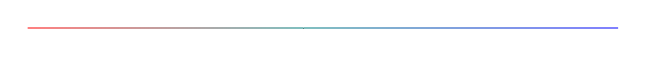
\begin{tikzpicture}
	\fill [left color=red!50, right color=teal!50] (0,0) rectangle (3.5,.01);
	\fill [left color=teal!50, right color=blue!50] (3.5,0) rectangle (7.5,.01);
	\end{tikzpicture}
\vspace{0.5cm}


%%%%%%%%%%%%%%%%%%%%%%%%%%%%%%%%%%%. \begin{ ------>. 
detsacado;  cuadro-naranja;  cuadro-gris;  miejercicio (solución extensa);  mipropuesto (solución corta y fuera del cuadro)

%%%%%%%%%%%%%%%%%%%%%%%%%%%%%%%%%%%. CURIOSIDAD
\vspace{1cm}
\color{ForestGreen!80}
\rule{250pt}{0.2pt}
Texto
\vspace{-8mm}
\begin{flushright}
\rule{250pt}{0.2pt}		
\end{flushright}	
\color{black}
\end{comment}







